\documentclass[12pt]{article}

\usepackage{graphicx}
\usepackage{paralist}
\usepackage{amsfonts}
\usepackage{amsmath}
\usepackage{hhline}
\usepackage{booktabs}
\usepackage{multirow}
\usepackage{multicol}
\usepackage{url}

\oddsidemargin -5mm
\evensidemargin -5mm
\textwidth 160mm
\textheight 200mm
\renewcommand\baselinestretch{1.0}

\usepackage[a4paper, total={6in, 8in}]{geometry}

\pagestyle {plain}
\pagenumbering{arabic}

\newcounter{stepnum}

%% Comments

\usepackage{color}

\newif\ifcomments\commentstrue

\ifcomments
\newcommand{\authornote}[3]{\textcolor{#1}{[#3 ---#2]}}
\newcommand{\todo}[1]{\textcolor{red}{[TODO: #1]}}
\else
\newcommand{\authornote}[3]{}
\newcommand{\todo}[1]{}
\fi

\newcommand{\wss}[1]{\authornote{blue}{SS}{#1}}

\title{Assignment 4, Design Specification}
\author{SFWRENG 2AA4}

\begin{document}

\maketitle
This Module Interface Specification (MIS) document contains modules, types and
methods for implementing the game \textit{2048}. At the start of the game, a board with dimensions of 4x4 will be generated on the board, making a total of 16 blank cells, with the exception of 2 randomly chosen independent cells which will spawn either a 2 or a 4.
\begin{itemize}
    \item While this is the base game, the following specification also allows for the functionality of a custom game board of a given integer dimension, as well as the functionality for the changing of the number from 2 and 4 to any integer and the double of the integer, to make the game more versatile and flexible. This also changes the winning condition for different number values; 2048 for 2, 3072 for 3, etc.
\end{itemize}
Every subsequent turn, one new cell, from the choice of the number n or the double of n with a chance of 90\% and 10\%, respectively, will be added to a blank cell. Every turn, the player will choose to slide all the tiles on the board in any of the 4 directions. A tile will continue moving in a direction until it is either stopped by the boundary, another tile of a different value, or a tile of the same value, in which case the two tiles will merge to form one tile with the value in the merged tile being the sum of the two merging tiles. A merged tile will similarly continue moving in a direction until it reaches the boundary or any other tile, regardless of the value. If a direction is made, but there is no room for any tiles to move or merges cannot be made, then that direction will not count as a move, and hence a new tile will not be added until a move that changes the board is made. This pattern continues until there are no valid moves left to play, or the player has made the 2048 tile. If there are no more valid moves left to play, it implies that the board is full of tiles, but there are no possible merges to be made, indicating that you are stuck and the game is over. If the 2048 tile is made, the player still has the option to continue the game until there are no more valid moves to play. The user is also given the option to quit or restart the game at any point in the game. The game can be launched and play by typing \texttt{make demo} in the terminal.

\newpage

\section{Overview of the design}

This design applies the Module View Specification (MVC) design pattern and the Singleton design pattern. The MVC components
are the \textit{GameController} (controller module), \textit{BoardT} (model module), and \textit{UserInterface} (view module).\\

The Singleton pattern is used, specified and implemented for \textit{GameController} and \textit{UserInterface}, where a single abstract object is created and is used throughout the game. This is applied by initializing the state variable for the object as null, and only creating a new object when it is null, otherwise returning the same object if it has already been created.

\medskip
The MVC design pattern is specified and implemented through the use of three distinct modules, namely \textit{BoardT, UserInterface,} and \textit{GameController}. The module \textit{BoardT} stores the state of the game board and the status of the game. The view module \textit{UserInterface} displays the state of the game board and game using text-based graphics. The controller \textit{GameController} is responsible for handling input actions, and combining the functionalities of the model and view components.

\medskip

\textit{GameController} and \textit{UserInterface}, use their respective getInstance() methods to obtain their abstract objects.\\

\newpage

The general outline for the Board that is represented in the game, along with the corresponding positions, is presented below.

\begin{center}
    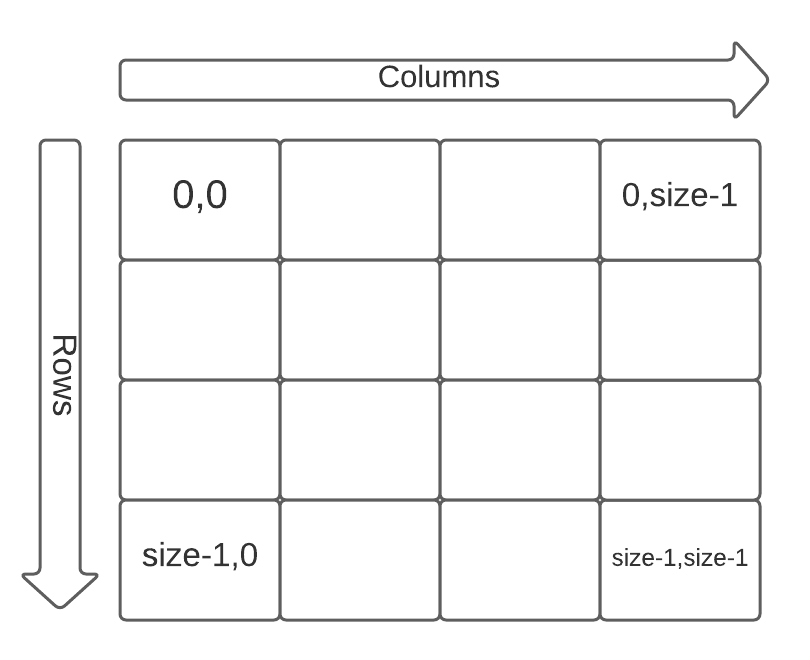
\includegraphics[width=0.5\textwidth]{Board_Diagram.png} \\
\end{center}

The general UML outline representations for the specification is given below

\begin{center}
    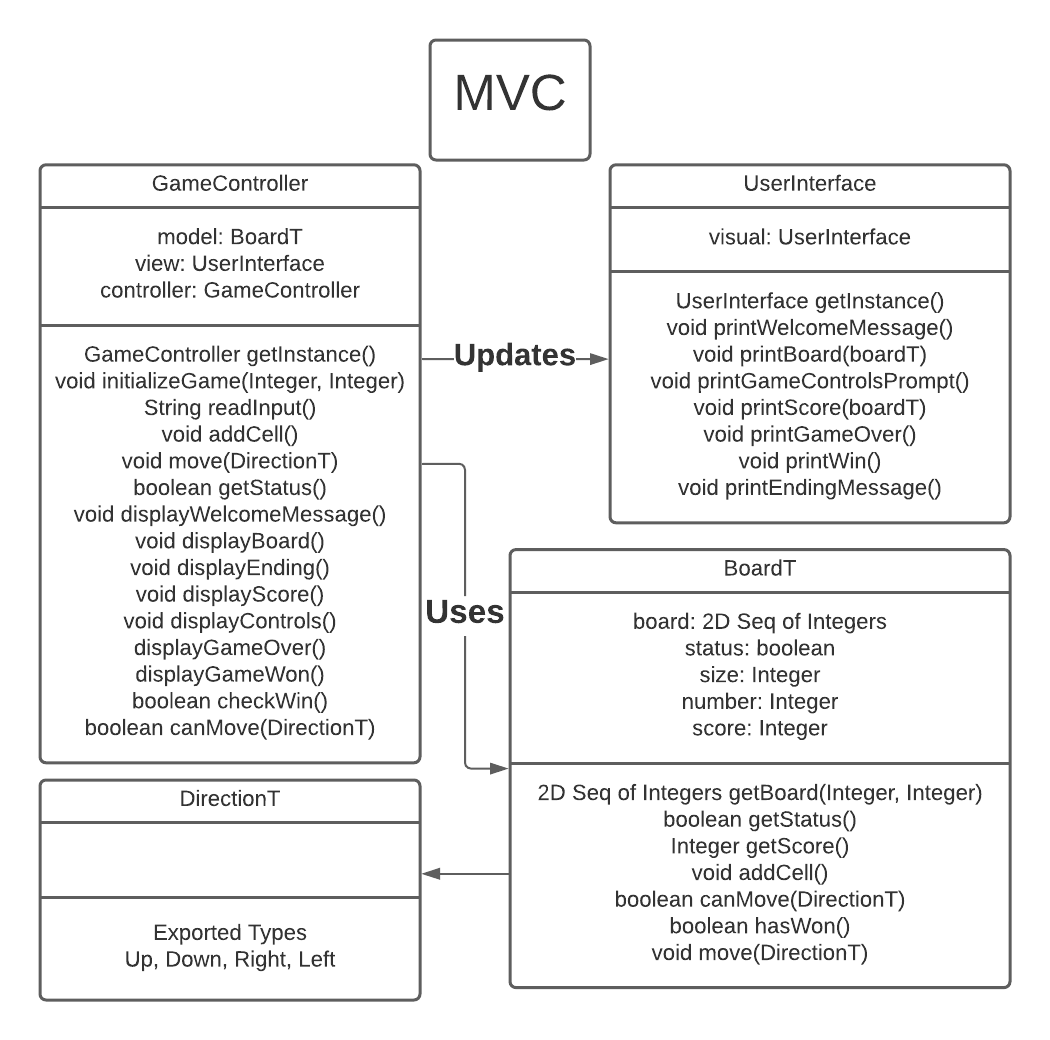
\includegraphics[width=0.75\textwidth]{UML_Diagram.png} \\
\end{center}

\newpage

\subsection*{Likely Changes my design considers:}

\begin{itemize}
  \item Data structure used for storing the game board
  \begin{itemize}
      \item Specifically, the game board must ideally be represented as a 2D array, which can be done using many implementations, and as such my design incorporates for any choice of such a data type, which could include nested lists, or specifically created 2D lists.
  \end{itemize}
  \item The size/dimensions of the board, are designed to be changeable by both the player and developer.
  \item The value of the number that the game is based off of is also designed to be changeable by both the user and developer for the purposes of creating a custom game.
  \item The visual representation of the game such as UI layout and the output board are designed to be dynamically changed for a given board.
  \item The input value taken by the user is designed to be modifiable and can be changed if the design specifications or usability of the game-play need to be changed.
  \item The aspect of adding new cells to the board was intentionally designed in such a way that a variable amount can be adjusted based on the requirments of the game.
  \item Change in the type of input that the user enters at runtime, this includes both the directional controls as well as the secondary options like quitting and restarting the game.
  \end{itemize}

\newpage

\section* {DirectionT Module}

\subsection*{Module}

Direction

\subsection* {Uses}

N/A

\subsection* {Syntax}

\subsubsection* {Exported Constants}

None

\subsubsection* {Exported Types}

DirectionT = \{Up, Down, Right, Left\}

\medskip

\noindent \textit{//These represent the 4 major directions that the player will move in}

\subsubsection* {Exported Access Programs}

None

\subsection* {Semantics}

\subsubsection* {State Variables}

None

\subsubsection* {State Invariant}

None

\newpage

\section* {Board ADT Module}

\subsection*{Template Module}

BoardT

\subsection* {Uses}

DirectionT

\subsection* {Syntax}

\subsubsection* {Exported Types}

BoardT = ?

\subsubsection* {Exported Constant}

None

\subsubsection* {Exported Access Programs}

\begin{tabular}{| l | l | l | l |}
\hline
\textbf{Routine name} & \textbf{In} & \textbf{Out} & \textbf{Exceptions}\\
\hline
new BoardT & $\mathbb{N}$, $\mathbb{N}$ & BoardT & \\
\hline
getBoard & ~ & seq of (seq of Integer) & \\
\hline
getStatus & ~ & $\mathbb{B}$ & \\
\hline
getScore & ~ & $\mathbb{N}$ & \\
\hline
canMove & DirectionT & $\mathbb{B}$ & \\
\hline
hasWon & ~ & $\mathbb{B}$ & \\
\hline
addCell & ~ & ~ &\\
\hline
move  & DirectionT &  ~  & \\
\hline
\end{tabular}

\subsection* {Semantics}

\subsubsection* {State Variables}

board: sequence [size, size] of $\mathbb{N}$ \\//This is to show that the board is a 2D array, can be implemented in many of ways\\
size: $\mathbb{N}$\\
number: $\mathbb{N}$\\
status: $\mathbb{B}$ \\
score: $\mathbb{N}$

\subsubsection* {State Invariant}

None

\subsubsection* {Assumptions}

\begin{itemize}
  \item The constructor BoardT is called for each object instance before any other access routine
  is called for that object.
  \item Assume there is a random function $random()$ that generates a random value between 0 and 1.
  \item Assume the $addCell()$ method is called after every valid turn/movement of the board.
  \item Assume the inputs will be of the correct type.
\end{itemize}

\subsubsection* {Design decision}

The board is stored in a 2D array, which is can be represented in many ways, but most commonly is the form of an array with a nested array. The board has inputs that will specify the dimensions of the board, where the rows are represented by each individual nested array, and the columns would be represented as the sequence at the same index values for all the nested arrays. As such the values stored in the board and the values represented correspondingly in the UI would coincide. For example in a 4x4 board, the value at the top left of the board in the UI at coordinate (0,0) would be the coordinate stored in the board, with the first 0 being the first row, and the second 0 being the second column. This allows for a very convenient and intuitive viewing of the board. The constructor was designed to have inputs for the board as this allows for a very large possibility of game configurations, and aims to increase user freedom and playability.

\subsubsection* {Access Routine Semantics}

new BoardT(gameSize, gameNumber):
\begin{itemize}
\item transition: \\
      size, number, status, score, $:=$ gameSize, gameNumber, true, 0\\\\
      board $:=$
      $\langle \begin{array}{c}
      \langle {0,...,0_{size-1}} \rangle\\
      .\\
      .\\
      .\\
      \langle {0,...,0_{size-1}} \rangle_{size-1}\\
      \end{array} \rangle$ \\
      board $:=$ addCell()\\
      board $:=$ addCell()

\item output: $out := \mathit{self}$
\item exception: None
\end{itemize}
//This method creates and initializes the board object with two randomly placed cells.\\

\noindent getBoard():
\begin{itemize}
\item transition: None
\item output: $out :=$ board
\item exception: None
\end{itemize}
//This method returns the board of the game.\\

\noindent getStatus():
\begin{itemize}
\item transition: status:= isPlayable()
\item output: $out :=$ status
\item exception: None
\end{itemize}
//This method gets the current status of the game.\\

\noindent getScore():
\begin{itemize}
\item transition: None
\item output: $out :=$ score
\item exception: None
\end{itemize}
\noindent //This method gets the current score of the game.\\

\noindent addCell():
\begin{itemize}
\item transition: $\neg \: (c = \langle \rangle) \Rightarrow setValue(c\:[0],\: c\:[1],\: randomValue())$\\
where $c = availableCell()$
\item output: None
\item exception: None
\end{itemize}
//This method adds a cell in any random, unfilled position on the board.\\

\noindent canMove($direction$):
\begin{itemize}
\item transition: None
\item output: $((((i : \mathbb{N} \: | \: i \in [0..size-1] \: |\: j : \mathbb{N} \:| \: j \in [0..size-1] \: | \: \neg \:(value = 0) \Rightarrow (
(direction = Direction.Up) \Rightarrow ((u = board[i][j]) \lor (u = 0)) \Rightarrow True)
\\(direction = Direction.Down) \Rightarrow ((d = board[i][j]) \lor (d = 0)) \Rightarrow True)
\\(direction = Direction.Right) \Rightarrow ((r = board[i][j]) \lor (r = 0)) \Rightarrow True)
\\(direction = Direction.Left) \Rightarrow ((l = board[i][j]) \lor (l = 0)) \Rightarrow True))
\\|(\:True \Rightarrow False)$
\\where $\\u = up(i,j),\: d = down(i,j),\: r = right(i,j),\: l = left(i,j)$
\item exception: None
\end{itemize}
//This method checks if a valid move can be made in a given direction, meaning that there are positions that are empty and can be filled by that movement.\\

\noindent hasWon():
\begin{itemize}
  \item transition: None
  \item output: $(i : \mathbb{N} \: | \: i \in [0..size-1] \: |\:j : \mathbb{N} \: | \: j \in [0..size-1] \: |\\ \:(board[i][j] \ge number*1024) \Rightarrow True) \:| \: True \Rightarrow False$
  \item exception: None
\end{itemize}
//This method checks if the player has won, specifically by checking if there is a winning tile or greater, depending on the game number, present on the board.\\\\
\noindent move(direction):
\begin{itemize}
\item transition: $((direction = Direction.Up) \Rightarrow moveUp() \:\\
| \: (direction = Direction.Down) \Rightarrow moveDown() \\
| \: (direction = Direction.Right) \Rightarrow moveRight() \\
| \: (direction = Direction.Left) \Rightarrow moveLeft())$
\item output: None
  \medskip
\end{itemize}
//This method performs the move operations by taking the respective direction and calling the appropriate function to perform the shift.

\newpage

\subsubsection* {Local Functions}

For the following 4 methods, namely moveUp, moveDown, moveRight, and moveLeft, the follwoing assumptions hold for the MIS spec. It is assumed that the three variables that are being gone through, namely h, i, and j, are being done in order, meaning all of j recurses for every single element of i, and every i recurses for every single element of h. Similarly, it is important to note that once an element is recursed over its entire length once, it will begin again until the variable prior to it has not reached its end. For example, j would recurse through its corresponding list of values for the first element of i's corresponding values. But once that is done, j must go over all of its elements again for i's second element in its corresponding values. This relationship holds for i and h as well. This ensures that we exhaust every possible combination of h,i,j possible, but in order, as these variables are used to traverse the board.\\
\\This allows us to check if the cell can be moved in a specific direction, and if so it is moved there, with the previous cell location becoming empty. This then continues for three iterations, as this allows for all possible movements to be made, as movements are made one step at a time, so at most we would need three iterations.\\

\noindent isPlayable: $void \rightarrow \mathbb{B}$:
\begin{itemize}
\item output: $(canMove(Direction.Up) \Rightarrow True \:\\
| \: canMove(Direction.Down) \Rightarrow True \\
| \: canMove(Direction.Right) \Rightarrow True \\
| \: canMove(Direction.Left) \Rightarrow True\\
| \: True \Rightarrow False)$
  \medskip
\end{itemize}
//This method checks if the game is still playable, meaning any move can be made in any of the 4 directions.\\

\noindent moveUp: $void \rightarrow void$
\begin{itemize}
    \item transition: $(h : \mathbb{N} \:|\: h \in [0..size-2] \:|\: i : \mathbb{N}\:|\: i \in [1..size-1] \:|\:  j : \mathbb{N}\:|\: j \in [0..size-1] \\
    \:|\: \neg\:(board[i][j] = 0) \Rightarrow \\
    \hspace{2cm} (
    (up(i,j) = 0)
    \Rightarrow setVal \\
    \:|\:
    (up(i,j) = board[i][j]) \: \land \: \neg \: (\langle i -1,j\rangle \in merged) \: \land \: \neg \: (\langle i,j \rangle \in merged)  \Rightarrow\\
    (merged \: || \: \langle \langle i -1,j\rangle \rangle) \: \land setVal \: \land score := score + (board[i][j] \:+\: up(i,j))))$
    \\\\where\\
    $setVal = setValue(i-1,j,board[i][j] + up(i,j)) \: \land \: setValue(i,j,0), \\merged = \langle \rangle \: (Initially)$
\end{itemize}
 //This method shifts all the cells in the board up on the following conditions that are stated in the MIS, as dictated by the rules of the game.\\

\noindent moveDown: $void \rightarrow void$
\begin{itemize}
    \item transition: $(h : \mathbb{N} \:|\: h \in [0..size-2] \:|\: i : \mathbb{N}\:|\: i \in [size-2..0] \:|\:  j : \mathbb{N}\:|\: j \in [0..size-1] \\
    \:|\: \neg\:(board[i][j] = 0) \Rightarrow \\
    \hspace{2cm} (
    (down(i,j) = 0)
    \Rightarrow setVal \\
    \:|\:
    (down(i,j) = board[i][j]) \: \land \: \neg \: (\langle i+1,j\rangle \in merged) \: \land \: \neg \: (\langle i,j \rangle \in merged)  \Rightarrow\\
    (merged \: || \: \langle \langle i+1,j\rangle \rangle) \: \land setVal \: \land score := score + (board[i][j] \:+\: down(i,j))))$
    \\\\where\\
    $setVal = setValue(i+1,j,board[i][j]) + down(i,j)) \: \land \: setValue(i,j,0), \\merged = \langle \rangle \: (Initially)$
\end{itemize}
//This method shifts all the cells in the board down on the following conditions that are stated in the MIS, as dictated by the rules of the game.\\
\medskip

\noindent moveRight: $void \rightarrow void$
\begin{itemize}
    \item transition: $(h : \mathbb{N} \:|\: h \in [0..size-2] \:|\: i : \mathbb{N}\:|\: i \in [0..size-1] \:|\:  j : \mathbb{N}\:|\: j \in [size-2..0] \\
    \:|\: \neg\:(board[i][j] = 0) \Rightarrow \\
    \hspace{2cm} (
    (right(i,j) = 0)
    \Rightarrow setVal \\
    \:|\:
    (right(i,j) = board[i][j]) \: \land \: \neg \: (\langle i,j+1\rangle \in merged) \: \land \: \neg \: (\langle i,j \rangle \in merged)  \Rightarrow\\
    (merged \: || \: \langle \langle i,j+1\rangle \rangle) \: \land setVal \: \land score := score + (board[i][j] \:+\: right(i,j))))$
    \\\\where\\
    $setVal = setValue(i,j+1,board[i][j] + right(i,j)) \: \land \: setValue(i,j,0), \\merged = \langle \rangle \: (Initially)$
\end{itemize}
//This method shifts all the cells in the board to the right on the following conditions that are stated in the MIS, as dictated by the rules of the game.\\\\
\medskip
\noindent moveLeft: $void \rightarrow void$
\begin{itemize}
    \item transition: $(h : \mathbb{N} \:|\: h \in [0..size-2] \:|\: i : \mathbb{N}\:|\: i \in [0..size-1] \:|\:  j : \mathbb{N}\:|\: j \in [1..size-1] \\
    \:|\: \neg\:(board[i][j] = 0) \Rightarrow \\
    \hspace{2cm} (
    (left(i,j) = 0)
    \Rightarrow setVal \\
    \:|\:
    (left(i,j) = board[i][j]) \: \land \: \neg \: (\langle i,j-1\rangle \in merged) \: \land \: \neg \: (\langle i,j \rangle \in merged)  \Rightarrow\\
    (merged \: || \: \langle \langle i,j-1\rangle \rangle) \: \land setVal \: \land score := score + (board[i][j] \:+\: left(i,j))))$
    \\\\where\\
    $setVal = setValue(i,j-1,board[i][j] + left(i,j)) \: \land \: setValue(i,j,0), \\merged = \langle \rangle \: (Initially)$
\end{itemize}
//This method shifts all the cells in the board to the left on the following conditions that are stated in the MIS, as dictated by the rules of the game.

\medskip

\noindent up: $\mathbb{N} \times \mathbb{N} \rightarrow \mathbb{N}$
\\ \noindent up($x, y$) $\equiv board\:[x+1][y]$\\
\medskip
//Returns the value at the top of a given position x,y.

\bigskip

\noindent down: $\mathbb{N} \times \mathbb{N} \rightarrow \mathbb{N}$
\\ \noindent down($x, y$) $\equiv board\:[x-1][y]$\\
\medskip
//Returns the value at the bottom of a given position x,y.

\bigskip

\noindent right: $\mathbb{N} \times \mathbb{N} \rightarrow \mathbb{N}$
\\ \noindent right($x, y$) $\equiv board\:[x][y+1]$\\
\medskip
//Returns the value to the right of a given position x,y.

\bigskip

\noindent left: $\mathbb{N} \times \mathbb{N} \rightarrow \mathbb{N}$
\\ \noindent left($x, y$) $\equiv board\:[x][y-1]$ \\
\medskip
//Returns the value to the left of a given position x,y.

\bigskip

\noindent availableCell: $void \rightarrow \textit{seq} \: \: \mathbb{N}$
\\availableCell $\equiv \neg \: (getZeroes(board) = \langle \rangle) \Rightarrow  (getZeroes(board) \: [position])$
\noindent \\where
$position = random() * |getZeroes(board)|$ such that $position$ rounds down to the nearest integer value.\\
\\//This method returns a coordinate position [x,y] in the form of a sequence, which is randomly chosen from all the coordinate positions from the sequence of positions that are obtained from getZeroes, which represents the empty cells on the board. This is used to spawn a new value at an empty cell.\\

\noindent setValue: $\mathbb{N} \times \mathbb{N} \times \mathbb{N}  \rightarrow void$
\\setValue $(x,y,value)$ $\equiv board := board[x][y] = value$\\
\medskip
\\//This method sets the value of the board at the given coordinate x,y, with given value.\\

\noindent randomValue(): $void \rightarrow \mathbb{N}$\\
randomValue(): $(random() < 0.9 \Rightarrow number \: | \: random() \ge 0.9 \Rightarrow number*2)$
\medskip
\\//This method returns a random value of either number or the double of number, with probabilities of 90\% and 10\% respectively.\\

\noindent getZeroes: seq [size] of seq [size] of $\mathbb{N} \rightarrow$ seq [size] of seq [size] of $\mathbb{N}$\\
getZeroes(arr):
\begin{itemize}
    \item transition := \\$(i : \mathbb{N} \: | \: i \in [0..size-1] \: | \: j : \mathbb{N} \: | \: j \in [0..size-1]\\ | \: ((arr [i] [j] = 0) \: \land \: \neg (\langle i,j \rangle \in zeroes)) \Rightarrow zeroes \: || \: \langle \langle i,j \rangle \rangle)$
    \item output := $zeroes$
\end{itemize}
\medskip
//Given a 2D array, this method finds all the positions of that 2D array that contain 0's.\\

\noindent setBoard: seq [size] of seq [size] of $\mathbb{N} \rightarrow$ seq [size] of seq [size] of $\mathbb{N}$\\
setBoard(arr):
\begin{itemize}
    \item transition : board := arr
\end{itemize}
\medskip
//Given a 2D array, this method sets the board of the $BoardT$ object to the 2D array. This method is not used in the implementation itself and is only used for testing.

\newpage

\section* {UserInterface Module}

\subsection* {UserInterface Module}

\subsection* {Uses}

None

\subsection* {Syntax}

\subsubsection* {Exported Types}

None

\subsubsection* {Exported Constants}

None

\subsubsection* {Exported Access Programs}

\begin{tabular}{| l | l | l | p{6cm} |}
\hline
\textbf{Routine name} & \textbf{In} & \textbf{Out} & \textbf{Exceptions}\\
\hline
getInstance & ~ & UserInterface &  \\
\hline
printBoard & BoardT & ~ & \\
\hline
printWelcomeMessage & ~ & ~ & \\
\hline
printGameControlsPrompt & ~ & ~ & \\
\hline
printScore & BoardT & ~ & \\
\hline
printGameOver & String & ~ & \\
\hline
printWin & ~ & ~ & \\
\hline
printEndingMessage & ~ & ~ & \\
\hline
\end{tabular}

\subsection* {Semantics}

\subsection*{Environment Variables}

window: A portion of computer screen to display the game and messages

\subsubsection* {State Variables}

visual: UserInterface

\subsubsection* {State Invariant}

None

\subsubsection* {Assumptions}

\begin{itemize}
\item The UserInterface constructor is called only once before any other access routines are called for that object.
\end{itemize}

\subsubsection* {Access Routine Semantics}

\noindent getInstance():
\begin{itemize}
  \item transition: visual $:=$ (visual = null $\Rightarrow$ new UserInterface())
  \item output: \textit{self}
  \item exception: None
\end{itemize}

\bigskip

\noindent printWelcomeMessage():
\begin{itemize}
\item transition: window $:=$ Prints a welcome message when user first enters the game.
\end{itemize}

\bigskip

\noindent printBoard(model):
\begin{itemize}
\item transition: window $:=$ Draws the game board onto the screen. All the elements of the board seq are iterated over, going row by row, from left to right. Because this is the same way that the values are actually stored in the board, this allows for an intuitive way of representing the board grid on the window. For example in a 4x4 board, the top left element in the board would be represented by the board at [0][0], and the bottom right would be represented by [3][3]. printBoard also adjusts the output of the board dynamically based on the size and game number. This is done to support a custom game functionality.
\end{itemize}

\bigskip

\noindent printGameControlsPrompt():
\begin{itemize}
\item transition: window $:=$\\ Prints a message showing the user the valid inputs to control the game.
\end{itemize}

\bigskip

\noindent printScore(model):
\begin{itemize}
\item transition: $(True \Rightarrow model.getScore())$\\
window $:=$ Prints the current score of the game, which happens after every turn.
\end{itemize}

\bigskip

\noindent printGameOver():
\begin{itemize}
\item transition: Prints the game over screen for when the player loses the game.
\end{itemize}

\bigskip

\noindent printWin():
\begin{itemize}
\item transition: Prints the game win screen for when the player wins the game.
\end{itemize}

\bigskip

\noindent printEndingMessage():
\begin{itemize}
\item transition: Prints the ending message thanking the user for playing after the game has concluded.
\end{itemize}

\subsubsection*{Local Function:}

spaces: $\mathbb{N}$ $\rightarrow$ void \\
spaces($l$) $\equiv$ $(i:\mathbb{N} \: | \: i \in [0..l-1]  \:| \: True \Rightarrow space)$\\
//Prints the specified amount of spaces.
\medskip

\noindent space: void $\rightarrow$ void\\
space: transition: window := Prints out a single space of empty string (` ').
\newpage

\section* {GameController Module}

\subsection* {GameController Module}

\subsection* {Uses}

BoardT, UserInterface

\subsection* {Syntax}

\subsubsection* {Exported Types}

None

\subsubsection* {Exported Constants}

None

\subsubsection* {Exported Access Programs}

\begin{tabular}{| l | l | l | p{4.7cm} |}
\hline
\textbf{Routine name} & \textbf{In} & \textbf{Out} & \textbf{Exceptions}\\
\hline
getInstance & BoardT, UserInterface & GameController & ~ \\
\hline
initializeGame & $\mathbb{N}, \mathbb{N}$ & ~ & ~\\
\hline
readInput & ~ & String & ~ \\
\hline
addCell & ~ & ~ & ~ \\
\hline
move & DirectionT & ~ & ~ \\
\hline
readGameModeInput & ~ & String & IllegalArgumentException \\
\hline
displayWelcomeMessage& ~ & ~ & ~ \\
\hline
getStatus & ~ & $\mathbb{B}$ & ~ \\
\hline
displayWelcomeMessage & ~ & ~ & ~ \\
\hline
displayBoard & ~ & ~ & ~ \\
\hline
displayEnding & ~ & ~ & ~ \\
\hline
displayControls & ~ & ~ & ~ \\
\hline
displayScore & ~ & ~ & ~ \\
\hline
displayGameOver & ~ & ~ & ~ \\
\hline
displayGameWon & ~ & ~ & ~ \\
\hline
checkWin & ~ & $\mathbb{B}$ & ~ \\
\hline
canMove & DirectionT & $\mathbb{B}$ & ~ \\
\hline
runGame & ~ & ~ & ~ \\
\hline
\end{tabular}

\subsection* {Semantics}

\subsection*{Environment Variables}

keyboard: Scanner(System.in) \qquad \textit{// reading inputs from keyboard}

\subsubsection* {State Variables}

model: BoardT \\
view: UserInterface \\
controller: GameController

\subsubsection* {State Invariant}

None

\subsubsection* {Assumptions}

\begin{itemize}
  \item It is assumed that the game will only be initiated and played through the running of the Game Controller, specifically by running make demo, as certain necessary aspects of the game logic, like adding cells, has been integrated into it.
  \item The GameController constructor is called only once before any other access routines are called for that object.
  \item It is assumed that both the model and view instances have already been initialized prior to the calling of the GameController constructor.
\end{itemize}

\subsubsection* {Access Routine Semantics}

getInstance($model$, $view$):
\begin{itemize}
  \item transition: controller $:=$ (controller = null $\Rightarrow$ new GameController ($m, v$))
  \item output: \textit{self}
  \item exception: None
\end{itemize}

\noindent initializeGame(size, number):
\begin{itemize}
  \item transition: model $:=$ $new BoardT(size, number)$
  \item output: None
  \item exception: None
\end{itemize}

\noindent readInput():
\begin{itemize}
  \item transition: None
  \item output: input:  String, entered from the keyboard by the User
  \item exception: None
\end{itemize}

\noindent addCell():
\begin{itemize}
  \item transition: model.board $:=$ (model.addCell())
  \item output: None
  \item exception: None
\end{itemize}

\noindent move($direction$):
\begin{itemize}
  \item transition: model.board $:=$ (model.move($direction$))
  \item output: None
  \item exception: None
\end{itemize}

\noindent getStatus():
\begin{itemize}
  \item transition: None
  \item output: $out$ $:=$ (model.getStatus())
  \item exception: None
\end{itemize}

\noindent displayWelcomeMessage():
\begin{itemize}
  \item transition: view $:=$ view.printWelcomeMessage()
\end{itemize}

\noindent displayBoard():
\begin{itemize}
  \item transition: view $:=$ view.printBoard()
\end{itemize}

\noindent displayEnding():
\begin{itemize}
  \item transition: view $:=$ view.printEndingMessage()
\end{itemize}

\noindent displayScore():
\begin{itemize}
  \item transition: view $:=$ view.printScore(model)
\end{itemize}

\noindent displayControls():
\begin{itemize}
  \item transition: view $:=$ view.printGameControlsPrompt()
\end{itemize}

\noindent displayGameOver():
\begin{itemize}
  \item transition: view $:=$ view.printGameOver()
\end{itemize}

\noindent displayGameWon():
\begin{itemize}
  \item transition: view $:=$ view.printWin()
\end{itemize}

\noindent checkWin():
\begin{itemize}
  \item output $:=$ model.hasWon()
\end{itemize}

\noindent canMove($direction$):
\begin{itemize}
  \item output $:=$ model.canMove($direction$)
\end{itemize}

\noindent runGame():
\begin{itemize}
  \item transition: Operational method for running the game. The game will start with a welcome message and display the list of controls for the user. The user will be prompted for either the choice of a regular game or a custom game. If the custom game option is chosen, then the user will specify certain values and boundaries for the input, otherwise a regular game will be chosen by default. After then prompting the user to press any button, it will then display the board and allow the user to play the game. The user can quit or restart the game whenever they would like. If the user wins, display a win message, otherwise, eventually, when the game ends, prompt a message asking the user to play another round or exit the game.
  \item output: None
\end{itemize}

\subsubsection*{Local Function:}

GameController: BoardT $\times$ UserInterface $\rightarrow$ GameController \\
GameController($model, view$) $\equiv$ new GameController($model, view$)

\newpage

\section*{Critique of Design}

\begin{itemize}
  \item BoardT was chosen to be an abstract data type module as opposed to an abstract object because this allows for a convenient way to reset and start the new game with a new instance of the board object if the player chooses to do so.
  \item The controller and view modules were chosen to be implemented as single abstract objects simply because only one instance of these objects are required to control the game, allowing the execution during runtime to become highly organized while avoiding any object conflicts that could possibly arise.
  \item Certain methods that are in the spec are decidedly unessential as they could easily be grouped into one function, but such methods were kept mainly due to keeping with the principles of abstraction and separation of concerns, meaning different methods deal with different levels of complexity for the same problem.
  \item One such example was that of the $addCell$, $availableCell$, and $getZeroes$ methods, which all perform together to spawn a random cell on the board. The reason they were separated was because each function deals with a specific area, $getZeroes$ determines all the possible locations where the new cell could be, $availableCell$ randomly finds one such cell from all these locations, and then $addCell$ adds the cell to the board with a value.
  \item Many of the print and display methods in the view and controller modules could be considered unessential, but are still included nonetheless mainly for the use of clarity and reusability, as most of these methods are called more than once and if they were to be implemented within the $runGame$ method, it would not look quite as understandable.
  \begin{itemize}
      \item That being said, within the GameController there are certain places where manual print statements are used directly in the code, but this is done only because these statements are done in a small portion at the beginning and are not repetitive.
  \end{itemize}

  \item Similarly, the $getCell$ and $setValue$ methods were not essential, as there functionalities could be directly implemented into the code they were used in, but they allowed for a very high level of usability and consistency in the code and allowed for a very streamlined development process.

  \item Both the spec and the code follow the principles of consistency one such example being in terms of variable and method names, which were kept consistent throughout. The use of objects names for the $BoardT$ and $UserInterface$ were kept to be model and view respectively. Similarly, variable names, such as coordinate positions, were kept to be i and j throughout, among other things.

  \item The DirectionT enum was specifically created to maintain the principle of generality, among other principles, within the code. Specifically, we can see the enum being used as an input to the move method, which determines which method to call in order to move the board. In a previous method of implementation, my specification was using 4 distinct methods for each specific direction, but the addition of the enum allowed me to define a more general $move$ method that would take in the direction parameter and call the specific move methods which can now remain private.

  \item The specification, as well as the resulting code implementation, were constructed using an incremental approach. For instance, when developing the move modules, it was initially specified so that there would be distinct modules that would perform individual movement features. This allowed for the focused design specification of these move modules which ensured their correctness. After they were made, the next incremental step was made to formulate a more general approach, which called for the inclusion of the $DirectionT$ datatype. This incremental approach which was followed in this situation, as well as many other places in the specification allowed for the correct and verifiable specification that can be seen now.

  \item Due to the nature of a game that generates random tiles at random positions, to test certain methods of the $BoardT$ module of the game, a method specifically created for testing was made in $BoardT$ that allows for the complete modification of the game board to set your own arrangement. Due to the potential power of this method, it is made protected only so it is accessible to the $TestBoardT$ module. Because this method allows for the setting of a custom board configuration, this allows me to specifically test my game for potentially problematic boundary or edge cases, as well as the correct functioning of the $move$ method.

  \item The inclusion of the $setBoard$ method, which was specifically made protected and is mentioned above, as well as the specifications as a whole were designed to follow the principle of information hiding. The state variables for all the modules were purposefully made private, with the inclusion of corresponding getter and setter methods so they could be individually accessed. Due to such practices, this prevents the properties of the individual data types to be manipulated, which could potentially result in problems or unexpected behavior.

  \item The test cases were specifically designed to validate the correctness of the program and specification based on the requirement, with the hopes of revealing any errors or unusual behavior during program execution. For that reason, every access routine in $BoardT$ is rigorously tested for full functionality based on the game requirements.

  \item For the testing of the board spawning functionality, and due to the nature of the randomness, the test case focuses on the existence of two generated cells for the board every time, rather than where and what cells are generated. Furthermore, it is important to note that the single spawn test that is created will technically be different every single time as it generates a new board object which could potentially be different. Nevertheless, the test case should and will always pass.
  \item No test cases were written for the UserInterface module as most of the methods were simple print statements to the terminal, which did not require testing. The $printBoard$ method was not feasible to create test-cases due to it's visual nature, therefore manual test cases were done to observe working functionality.
  \item No test cases were written for the GameController module as nearly all of the methods were dependant on methods from the view and model modules. Furthermore it was not feasible to write any form of test cases for the $runGame$ method, and instead it was tested manually.

  \item It is to be noted that while my game contains support for the changing of both the board size and values, the test cases that are present only test the functionality of the base game, specifically a 4x4 board with values spawning between 2 and 4. This is mainly due to the fact that it would be troublesome to test the functionality of a potentially infinite amount of game variations.

  \item While my relaxed implementation of the game 2048 allows for a large degree of customization, a potential design flaw that I did not factor into my design may have also resulted from such an implementation. The base game 2048 allows for a very unique and balanced experience as the powers of two are also their doubles. This would mean that doubling values would never result in numbers like 6 that are multiples of 2, but not powers. This is not the same case for other numbers and as such, this could lead to unexpected difficulty spikes that cannot be accounted for without proper testing. As such, for numbers that are not 2, while the game might still be playable and winnable, it might not be as balanced as simple 2048.

  \item While the custom game functionality implementation of the game 2048 allows for a potentially large number of both board and number variations, due to the possible unexpected possibilities in terms of both gameplay and implementation for these numbers, the users options for both the board size and number have been limited to a modest range. This was also done to preserve the actual playability of the game as numbers or board sizes higher than the ones given might not be as visually or game-play appealing.

  \item It is to be noted that there are methods in my specification that are designed to violate the principles of minimality. The $move$ method, as well as its complementing local functions, clearly violate minimality by changing transitions for multiple state variables, namely $board$ and $status$. This was done, however, to provide a seamless and appropriate location to update the score as the score was only updated when tiles were moved and merged, and it made sense to include it there. Similarly, the $runGame$ method in the Controller is not minimal as it does multiple transitions and essentially controls the entire game. This however could not be avoided as a single method was needed to accomplish all these transitions for understandability and completeness.

  \item Many, if not all, of my functions were designed to incorporate the principle of anticipation of change, specifically through maintainability. As many of the methods were quite general and minimal, this potentially allows for any changes made in the requirements to be easily editable in the specification and design, with a very minimal amount of changes. This can clearly be seen through the use of the two state variables, $size$ and $number$, that are used throughout the specification to keep uniformity.

  \item Furthermore, the use of the model, view, controller design technique, or the MVC, also makes my design maintainable, which reduces risk when making changes. MVC modularizes the specification by abstracting the functionalities into three
        components. These components are the model, which encapsulates the internal data and status of the game, the view, which displays the state of the game, and the controller, which handles
        the input actions to execute related actions to respond to events. Through the MVC, if anything would need to be changed in the model component, for example, we can be certain that these changes will not affect the working functionality of the view or controller modules, and vice versa.
  \item The MVC design strategy also supports high cohesion in the entire project as a whole. High cohesion is maintained mainly in part from the grouping of related functionalities within each module. That is to say that each module focuses on a specific aspect of the project that has been abstracted from the other components.

  \item The MVC design also supports low coupling mainly due to the fact of the independence of the three modules from one another. Each of these modules focus on a unique and distinct aspect of the game as a whole, with the $BoardT$ dealing with the game setup and logic, the UserInterface dealing with the display and visuals, and the controller dealing with the inputs and integrating them with the visuals and game logic. This translates in the useful quality of minimal conflict between the modules and their changes, and allows for the developer to not have to worry about unnecessary aspects of design when implementing one of these modules.

  \item The use of the Singleton design pattern can be clearly seen in the implementation of the UserInterface and GameController methods. The use of a single object to design these modules, as opposed to a data type, allowed for a simpler design focus and less clutter, as there need not be more than one UserInterface or GameController active at one time, as opposed to certain situations with boards where you may need multiple instances of them.

\end{itemize}

\newpage

\section*{Answers to Questions:}

Q1: Draw UML diagrams for the modules in Assignment 3.

\bigskip

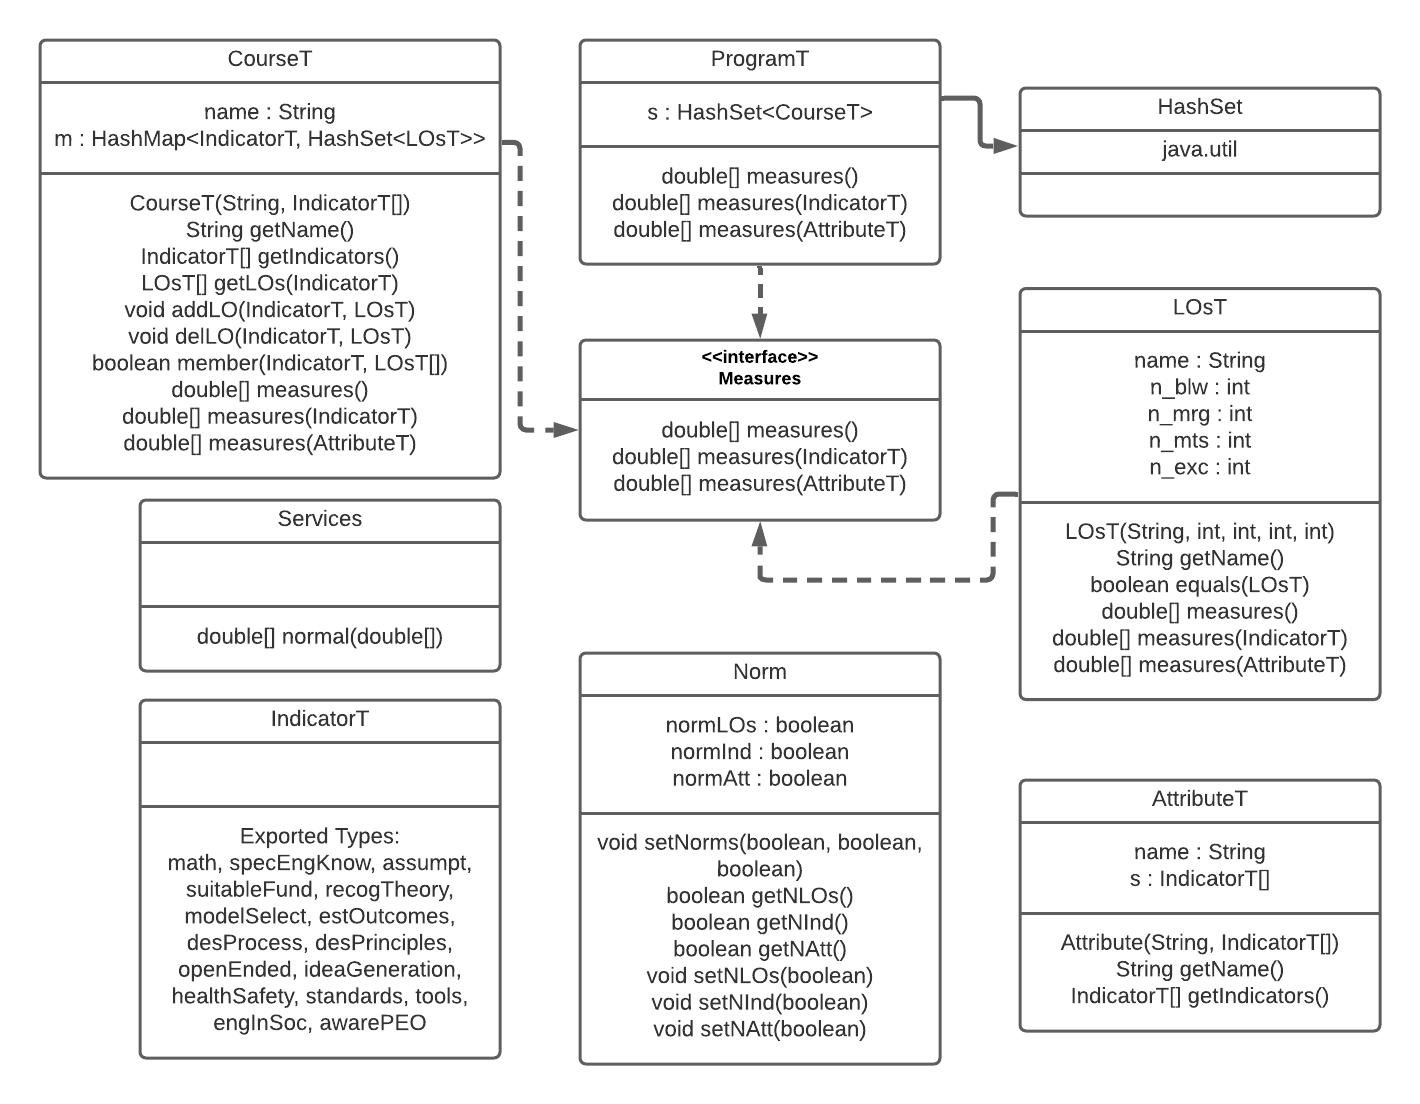
\includegraphics[width=1\textwidth]{Q1_UML_Diagram.png} \\

\end{document}
